\documentclass[11pt,a4paper,openany]{book}

\usepackage[utf8]{inputenc}
\usepackage{amsmath,amssymb,amsthm,bm,mathtools}
\usepackage{geometry}
\geometry{a4paper, margin=1.8cm, top=2.2cm, bottom=2.2cm}
\usepackage{booktabs}
\usepackage{array}
\usepackage{longtable}
\usepackage{tikz}
\usetikzlibrary{calc,shapes.geometric,patterns,arrows.meta,positioning}
% mosaic_tikz_preamble.tex - Strict Two-Colour Symmetry Taxonomy for Composition Mosaics
%
% Colour Taxonomy:
%   - Symmetric / Reversible Compositions: mosaicblue (blue!30)
%   - Chiral / Non-Symmetric Compositions: mosaicpink (red!25)
%   - Opacity: fill opacity=0.65 for all polygon fills to enable interpenetration visibility.

\usepackage{tikz}
\usetikzlibrary{shapes.geometric, calc}

% Strict Two-Colour Taxonomy Definitions
\colorlet{mosaicblue}{blue!30}
\colorlet{mosaicpink}{red!25}

% TikZ Styles
\tikzset{
  % Standard uniform shell polygon size across all figures
  mosaic shell/.style={
    regular polygon,
    minimum size=1.8cm,
    draw=gray!40,
    thick
  },
  mosaic core shell/.style={
    regular polygon,
    minimum size=1.8cm,
    draw=gray!60,
    thick,
    densely dashed
  },
  mosaic polygon/.style={
    regular polygon,
    minimum size=1.8cm,
    draw=gray!40,
    thick
  },
  % Partition blocks
  symmetric block/.style={
    black, thick, fill=mosaicblue, fill opacity=0.65
  },
  chiral block/.style={
    black, thick, fill=mosaicpink, fill opacity=0.65
  },
  % Composition transversals (dashed paths)
  symm transversal/.style={
    blue!80!black,
    line width=1.5pt,
    dashed
  },
  symm dot/.style={
    fill=blue!80!black
  },
  chiral transversal/.style={
    red!75!black,
    line width=1.5pt,
    dashed
  },
  chiral dot/.style={
    fill=red!75!black
  },
  % Vertex coordinate discs and size badges
  active disc/.style={
    circle,
    fill=white,
    draw=black!70,
    line width=0.6pt,
    text=black,
    font=\tiny\bfseries,
    inner sep=1.0pt
  },
  pin dot/.style={
    circle,
    fill=white,
    draw=black!70,
    line width=0.6pt,
    text=black,
    font=\tiny\bfseries,
    inner sep=1.0pt
  },
  symm size badge/.style={
    circle,
    fill=mosaicblue,
    draw=blue!80!black,
    line width=0.6pt,
    text=blue!90!black,
    font=\tiny\bfseries,
    inner sep=0.7pt
  },
  chiral size badge/.style={
    circle,
    fill=mosaicpink,
    draw=red!75!black,
    line width=0.6pt,
    text=red!90!black,
    font=\tiny\bfseries,
    inner sep=0.7pt
  },
  coupling arrow/.style={
    ->,
    >=stealth,
    line width=1.1pt,
    shorten <=4pt,
    shorten >=4.5pt
  },
  inactive dot/.style={
    circle,
    fill=black!25,
    inner sep=1.0pt
  },
  mono size badge/.style={
    symm size badge
  },
  unigon dot/.style={
    black,
    fill=mosaicblue,
    line width=0.8pt
  },
  digon stroke/.style={
    line width=3.2pt,
    line cap=round
  },
  digon lens/.style={
    fill=mosaicblue,
    fill opacity=0.75,
    draw=blue!75!black,
    line width=0.8pt
  }
}

\usepackage{csquotes}
\MakeOuterQuote{"}
\usepackage{placeins}
\usepackage{pdfpages}

\usepackage{hyperref}
\hypersetup{
  pdftitle={The Atlas of Hexadecagonal Compositions: Affine Macro-Orbits of Composition Mosaics on Z16},
  pdfauthor={Gemma Knee and Antigra Vitti},
  colorlinks=true,
  linkcolor=blue!70!black,
  citecolor=blue!70!black,
  urlcolor=blue!70!black
}

\title{\textbf{\Huge The Atlas of Hexadecagonal Compositions}\\[0.4cm] {\Large\itshape Affine Macro-Orbits of Composition Mosaics on \texorpdfstring{$\mathbb{Z}_{16}$}{Z16}}}
\author{Gemma Knee \and Antigra Vitti}
\date{November 2026}

% Custom Theorem Styles without terminating punctuation bacilli
\newtheoremstyle{breakdef}%
  {9pt}% Space above
  {9pt}% Space below
  {\normalfont}% Body font
  {0pt}% Indent amount
  {\bfseries}% Theorem head font
  {}% Punctuation after theorem head
  {\newline}% Space after theorem head
  {\thmname{#1}\thmnumber{ #2}\thmnote{ (#3)}}% Head spec

\newtheoremstyle{breakthm}%
  {9pt}% Space above
  {9pt}% Space below
  {\itshape}% Body font
  {0pt}% Indent amount
  {\bfseries}% Theorem head font
  {}% Punctuation after theorem head
  {\newline}% Space after theorem head
  {\thmname{#1}\thmnumber{ #2}\thmnote{ (#3)}}% Head spec

\theoremstyle{breakthm}
\newtheorem{theorem}{Theorem}[chapter]
\newtheorem{proposition}[theorem]{Proposition}
\newtheorem{corollary}[theorem]{Corollary}
\newtheorem{lemma}[theorem]{Lemma}

\theoremstyle{breakdef}
\newtheorem{definition}[theorem]{Definition}
\newtheorem{example}[theorem]{Example}
\newtheorem{remark}[theorem]{Remark}

\numberwithin{equation}{chapter}

\begin{document}

\frontmatter

\begin{titlepage}
\centering
\vspace*{0.8cm}
{\Huge \bfseries The Atlas of\\[0.35cm] Hexadecagonal Compositions\par}
\vspace{0.45cm}
{\Large\itshape Affine Macro-Orbits of Composition Mosaics on $\mathbb{Z}_{16}$\par}
\vspace{0.6cm}
\rule{0.35\textwidth}{0.8pt}\par
\vspace{0.6cm}
{\Large Gemma Knee \qquad Antigra Vitti\par}
\vspace{0.8cm}

\input{tkz/fig_cover_t10360.tkz}

\vfill
\vspace*{0.4cm}
\end{titlepage}

% Preface.tex - Preface to The Atlas of Hexadecagonal Compositions
% Author: Gemma Knee & Antigra Vitti

\chapter*{Preface}
\addcontentsline{toc}{chapter}{Preface}

This atlas presents an exhaustive structural and visual census of the composition mosaics on the cyclic lattice $\mathbb{Z}_{16}$. At its foundation lies a classical combinatorial problem: partitioning the sixteen vertices of a regular hexadecagon into four disjoint blocks of four vertices each. Across the discrete universe, exactly $2{,}627{,}625$ such partitions exist. When viewed under Euclidean translations and reflections, these configurations coalesce into $83{,}488$ dihedral orbits, each defining a geometric mosaic of four inscribed quadrilaterals whose edge strides sum to sixteen.

The purpose of this volume is to document the deeper multiplicative architecture that governs these geometric forms. Under the action of the affine group $\operatorname{Aff}(\mathbb{Z}_{16}) = \mathbb{Z}_{16} \rtimes \mathbb{Z}_{16}^\times$, the modular multipliers act as an outer Galois symmetry group $C_4 \cong \mathbb{Z}_{16}^\times / \{\pm 1\}$. Driven by the prime multiplier $\mu_3 \colon x \mapsto 3x \pmod{16}$, the $83{,}488$ dihedral orbits assemble into exactly $21{,}030$ affine macro-orbits:
\begin{itemize}
  \item $20{,}721$ \textbf{Tetramers}: 4-cycles undergoing periodic cycling under $\mu_3$
  \item $295$ \textbf{Dimers}: 2-cycles invariant under squared dilation $\mu_9 = \mu_3^2$
  \item $14$ \textbf{Monomers}: singular fixed points possessing full affine invariance
\end{itemize}

Throughout the atlas, every mosaic is rendered according to a strict two-colour taxonomy grounded in block symmetry. A block whose chord strides are invariant under reflection is shaded in blue, whilst a chiral block lacking internal bilateral symmetry is shaded in pink. The cover artwork portrays the median tetramer $T_{10360}$, situated halfway through the tetramer catalogue. Possessing orbit size $|O|=32$, signature $[nsnn]$, and Dirichlet energy $E=614$, its single symmetric block coexists with three chiral blocks in a perpetual four-phase dance under $\mu_3$.

In addition to pure combinatorial geometry, these configurations offer immediate interpretations in musical voice leading, pitch-class set polyphony, and rhythmic partitioning. The accompanying computational suite, including the command-line utility \texttt{midipartner} and the complete electronic index tables, permits researchers and composers to explore the sonic and algebraic properties of every macro-orbit.

\vspace{1.5cm}
\noindent
\begin{flushright}
\textit{Gemma Knee} \qquad \textit{Antigra Vitti}\\[0.25cm]
\textit{Newcastle upon Tyne}\\[0.15cm]
\textit{November 2026}
\end{flushright}


\tableofcontents

\mainmatter

\chapter{Geometry}
\label{chap:geometry}
\section{Hexadecagonal Architecture}
\label{sec:introduction}

The sixteen vertices of the cyclic lattice $\mathbb{Z}_{16}$ give rise to an immense combinatorial landscape. When we partition the regular hexadecagon into four disjoint blocks of four vertices each (the shape $z_4^4$), the vertices connect to form inscribed polygons whose cyclic edge strides define integer compositions of $16$ (following Fripertinger and Kerber). 

Across the full combinatorial universe, exactly $2{,}627{,}625$ distinct set partitions tile the sixteen vertices into four quadrilaterals:
\begin{equation}
\label{eqn:raw-universe-z44}
|\mathcal{P}(z_4^4)| = \frac{1}{4!} \binom{16}{4} \binom{12}{4} \binom{8}{4} \binom{4}{4} = 2{,}627{,}625
\end{equation}
Under the physical symmetries of the polygon—the translations and reflections generating the dihedral group $D_{16}$ of order $32$—these configurations gather into the graded bivariate orbit polynomial:
\begin{equation}
\label{eqn:orbit-poly-d16}
P_{16}(z_4^4, \omega) = 80802\omega^{32} + 2568\omega^{16} + 102\omega^{8} + 13\omega^{4} + 2\omega^{2} + \omega^{1}
\end{equation}
Evaluating this polynomial at $\omega = 1$ reveals the total census of non-equivalent dihedral mosaic orbits:
\begin{equation}
\label{eqn:total-d16-orbits}
P_{16}(z_4^4, 1) = 80802 + 2568 + 102 + 13 + 2 + 1 = 83{,}488
\end{equation}

Beneath this vast collection of 83 thousand geometric configurations lies a deeper, unifying algebra governed by modular multiplication. The affine group $\operatorname{Aff}(\mathbb{Z}_{16}) = \mathbb{Z}_{16} \rtimes (\mathbb{Z}_{16})^\times$ acts on the polygon not merely by turning or flipping it, but by dilating its chords through modular unit multipliers.

The outer automorphism group $G_{\text{macro}} = \operatorname{Aff}(\mathbb{Z}_{16}) / D_{16} \cong C_4$ acts upon the dihedral orbits as a cyclic permutation group of order $4$, driven by the Galois multiplier $\mu_3 \colon x \mapsto 3x \pmod{16}$. This multiplicative symmetry weaves the $83{,}488$ individual dihedral mosaics into exactly $21{,}030$ Affine Macro-Orbits.

\subsection{Lattice Geometry and Clock-Face Orientation}
\label{sec:clock-face-orientation}

Across all diagrams, plates, and catalogue listings in this atlas, the sixteen hexadecagonal vertices are identified as $\{0, 1, \dots, 15\}$ according to a clock-face geometry with $0$ at the top, advancing by $1$ clockwise.

A representative partition of the set of vertices as a \textit{mosaical shape} $z_4^4$ is exemplified by $P = \{\{0, 2, 7, 9\}, \{1, 4, 10, 11\}, \{3, 8, 12, 15\}, \{5, 6, 13, 14\}\}$.

A perimeter \textit{stride} between successive vertices of an inscribed block $B = \{v_1, v_2, v_3, v_4\}$ (ordered circularly $v_1 < v_2 < v_3 < v_4$) is defined as the forward modular step around the polygon, $s_i = (v_{i+1} - v_i) \bmod 16$ (where $v_5 \equiv v_1$) such that $\sum_{i=1}^4 s_i = 16$. For example, the first of the four blocks of our exemplar $P$, above, has strides $(2 - 0)$, $(7 - 2)$, $(9 - 7)$, $(0 - 9)$---which is to say $2, 5, 2, 7$ since $7 \equiv -9 \pmod{16}$---notice that $2 + 5 + 2 + 7 = 16$ as required.

Figure~\ref{fig:clock-face-convention} below illustrates vertex numbering, the entire example partition $P$, the vertices of the first block of $P$, and finally the strides of that first block.

\begin{figure}[htbp]
\centering
\input{tkz/T00646.tkz}
\caption{\label{fig:clock-face-convention}$z_4^4$-mosaic $P$ on $\mathbb{Z}_{16}$, with its modular arithmetic}
\end{figure}

The other three blocks of $P$ have corresponding strides $3 + 6 + 1 + 6$, $5 + 4 + 3 + 4$, and $1 + 7 + 1 + 7$.

Mosaics will generally be abbreviated (to save space) using hexadecimal numerals where $\mathrm{A}=10$, $\mathrm{B}=11$, $\mathrm{C}=12$, etc. For instance, the mosaic $P$ above is notated as \path{/0279/14AB/38CF/56DE/}, using lexicographical ordering to determine a \textit{canonical representative} of dihedrally equivalent partitions (mosaics).

\section{Affine Macro-Orbit Theory on \texorpdfstring{$\mathbb{Z}_{16}$}{Z16}}
\label{sec:affine-macro-orbits}

\subsection{The Outer Galois Multiplier Group}

Let $\operatorname{Aff}(\mathbb{Z}_n) = \{x \mapsto ax + b \pmod n \mid a \in (\mathbb{Z}_n)^\times, b \in \mathbb{Z}_n\}$ denote the affine group of the cyclic ring $\mathbb{Z}_n$. The dihedral group $D_n = \{x \mapsto \pm x + b \pmod n\}$ is a normal subgroup of $\operatorname{Aff}(\mathbb{Z}_n)$. Consequently, the outer quotient group:
\begin{equation}
\label{eqn:g-macro-def}
G_{\text{macro}} = \operatorname{Aff}(\mathbb{Z}_n) / D_n \cong (\mathbb{Z}_n)^\times / \{\pm 1\}
\end{equation}
acts naturally as a group of permutations on the set of $D_n$-orbits of composition mosaics.

\begin{proposition}[Cyclic Structure of the Macro-Group on $\mathbb{Z}_{16}$]
\label{prop:g-macro-c4}
For $n = 16$, the unit group $(\mathbb{Z}_{16})^\times = \{1, 3, 5, 7, 9, 11, 13, 15\}$ is isomorphic to $C_2 \times C_4$. Factoring out the reflection subgroup $\{\pm 1\} = \{1, 15\}$, the quotient group is cyclic of order $4$:
\begin{equation}
\label{eqn:c4-quotient}
G_{\text{macro}} \cong C_4 = \langle \mu_3 \rangle
\end{equation}
generated by the Galois dilation multiplier:
\begin{equation}
\label{eqn:mu3-def}
\mu_3 \colon \mathbb{Z}_{16} \to \mathbb{Z}_{16}, \quad x \mapsto 3x \pmod{16}
\end{equation}
\end{proposition}

\begin{proof}
The cosets of $(\mathbb{Z}_{16})^\times$ modulo $\{1, 15\}$ are:
\begin{enumerate}
    \item $C_0 = \{1, 15\}$ (identity)
    \item $C_1 = \{3, 13\}$
    \item $C_2 = \{7, 9\}$
    \item $C_3 = \{5, 11\}$
\end{enumerate}
Under multiplication modulo $16$, $3^1 \equiv 3 \in C_1$, $3^2 = 9 \equiv -7 \in C_2$, $3^3 = 27 \equiv 11 \equiv -5 \in C_3$, and $3^4 = 81 \equiv 1 \in C_0$. Thus $C_1$ has order $4$, generating the cyclic quotient $C_4$.
\end{proof}

The unique order-2 subgroup of $G_{\text{macro}}$ is generated by the involution:
\begin{equation}
\label{eqn:mu7-involution}
\mu_7 \colon x \mapsto 7x \equiv -9x \pmod{16}
\end{equation}
which corresponds to the intermediate affine subgroup:
\begin{equation}
\label{eqn:h2-subgroup}
H_2 = D_{16} \rtimes \langle \mu_7 \rangle \le \operatorname{Aff}(\mathbb{Z}_{16})
\end{equation}
of order $64$, whose unit set is $\{1, 7, 9, 15\}$.

We demonstrate such an $x \mapsto 3x \pmod{16}$ inflation with the first block in our example mosaic, $P$, above. This block is the subset $\{0, 2, 7, 9\}$ and is dilated (or inflated) by multiplying each vertex number by $3$, yielding $\{0, 6, 21, 27\}$. The last two elements---having been inflated round the clock, as it were---are not in our ground set except as vertices $5$ and $11$ (via modular arithmetic). So the dilated shape is now the subset $\{0, 5, 6, 11\}$---clearly not the same shape. Dilating again produces $0, 15, 18, 33$---the subset $\{0, 1, 2, 15\}$---and a third dilation yields $0, 3, 6, 45$, i.e.\ $\{0, 3, 6, 13\}$. We know, from the proof above, that a fourth dilation (having come this far without return) \textit{must} return us to the beginning, and $0, 9, 18, 39$---being (modulo $16$) the set $\{0, 2, 7, 9\}$---is indeed that first subset.

Figure~\ref{fig:inflation-in-action} below illustrates the four dilations of the first subset of partition $P$.

\begin{figure}[htbp]
\centering
\input{tkz/T00646-1-dil.tkz}
\caption{\label{fig:inflation-in-action}Successive inflations of subset $\{0, 2, 7, 9\}$}
\end{figure}

The second block of $P$ is $\{1, 4, 10, 11\}$, which maps to numbers $3, 12, 30, 33$---the subset $\{1, 3, 12, 14\}$---which maps again to $3, 9, 36, 42$---the subset $\{3, 4, 9, 10\}$. This maps, for the third time, to $9, 12, 27, 30$---the subset $\{9, 11, 12, 14\}$---which maps for the fourth (and perforce last) time to $27, 33, 36, 42$---the subset $\{1, 4, 10, 11\}$, which is the inevitable second block of $P$ again. The reader should verify that the remaining two blocks, i.e.\ $\{3, 8, 12, 15\}$ and $\{5, 6, 13, 14\}$, perform the same way, and also that at no point in any of the four dilations do the subsets intersect, meaning each stage produces a genuine partition of $\mathbb{Z}_{16}$.

\subsection{Burnside Spectral Decomposition}

Because $G_{\text{macro}} \cong C_4$ acts on the $83{,}488$ dihedral orbits, orbit lengths must divide $|C_4| = 4$. Every affine macro-orbit is therefore one of three types:
\begin{enumerate}
    \item \textbf{Monomers (Size 1)}: Fixed points invariant under all multipliers $\mu_3, \mu_5, \mu_7$.
    \item \textbf{Dimers (Size 2)}: 2-cycles invariant under the involution $\mu_7$, but transposed by $\mu_3 \leftrightarrow \mu_5$.
    \item \textbf{Tetramers (Size 4)}: Full 4-cycles under $\mu_3$:
    \[
    O \xrightarrow{\mu_3} \mu_3(O) \xrightarrow{\mu_3} \mu_7(O) \xrightarrow{\mu_3} \mu_5(O) \xrightarrow{\mu_3} O
    \]
\end{enumerate}

\begin{theorem}[Spectral Decomposition Theorem for $z_4^4$]
\label{thm:spectral-decomposition-z44}
Under the action of $G_{\text{macro}} \cong C_4$, the $83{,}488$ dihedral orbits of shape $z_4^4$ on $\mathbb{Z}_{16}$ decompose into exactly $21{,}030$ Affine Macro-Orbits, comprising:
\begin{itemize}
    \item $c_1 = 14$ monomers (size 1 fixed points)
    \item $c_2 = 295$ dimers (size 2 cycles)
    \item $c_4 = 20{,}721$ tetramers (size 4 cycles)
\end{itemize}
satisfying:
\begin{equation}
\label{eqn:spectral-sum}
c_1 \times 1 + c_2 \times 2 + c_4 \times 4 = 14 + 590 + 82{,}884 = 83{,}488
\end{equation}
and:
\begin{equation}
\label{eqn:total-macro-sum}
c_1 + c_2 + c_4 = 14 + 295 + 20{,}721 = 21{,}030
\end{equation}
\end{theorem}

\begin{proof}
Let $X$ denote the set of $2{,}627{,}625$ raw partitions of $\mathbb{Z}_{16}$ of shape $z_4^4$. The group $\operatorname{Aff}(\mathbb{Z}_{16})$ acts on $X$. The $128$ group elements partition into $9$ cycle classes in the symmetric group $S_{16}$. For each permutation $g \in \operatorname{Aff}(\mathbb{Z}_{16})$, the number of invariant set partitions $|\operatorname{Fix}_X(g)|$ is determined by cycle compatibility between $g$ and the block permutations in $S_4$:
\begin{center}
\begin{tabular}{llrr}
\toprule
Cycle Class of $g \in S_{16}$ & Elements in $\operatorname{Aff}_{16}$ & Fixed Partitions $|\operatorname{Fix}_X(g)|$ \\
\midrule
$(1^{16})$ & $1$ (identity) & $2{,}627{,}625$ \\
$(1^8, 2^4)$ & $2$ & $5{,}425$ \\
$(2^8)$ & $9$ & $4{,}025$ \\
$(1^2, 2^7)$ & $16$ & $945$ \\
$(4^4)$ & $12$ & $89$ \\
$(1^2, 2^3, 4^2)$ & $16$ & $33$ \\
$(1^4, 2^2, 4^2)$ & $8$ & $29$ \\
$(8^2)$ & $32$ & $5$ \\
$(16^1)$ & $32$ & $1$ \\
\bottomrule
\end{tabular}
\end{center}
Applying Burnside's Lemma:
\begin{enumerate}
    \item Dihedral group $D_{16}$ (order $32$, units $\{1, 15\}$):
    \[
    N_{D_{16}} = \frac{1}{32} \sum_{g \in D_{16}} |\operatorname{Fix}_X(g)| = 83{,}488
    \]
    \item Intermediate subgroup $H_2$ (order $64$, units $\{1, 7, 9, 15\}$):
    \[
    N_{H_2} = \frac{1}{64} \sum_{g \in H_2} |\operatorname{Fix}_X(g)| = 42{,}046
    \]
    \item Full affine group $\operatorname{Aff}_{16}$ (order $128$, all $8$ units):
    \[
    N_{\operatorname{Aff}_{16}} = \frac{1}{128} \sum_{g \in \operatorname{Aff}_{16}} |\operatorname{Fix}_X(g)| = 21{,}030
    \]
\end{enumerate}
The orbit counts under $D_{16}$, $H_2$, and $\operatorname{Aff}_{16}$ satisfy the linear system:
\[
\begin{cases}
c_1 + 2c_2 + 4c_4 = 83{,}488 \\
c_1 + 2c_2 + 2c_4 = 42{,}046 \\
c_1 + c_2 + c_4 = 21{,}030
\end{cases}
\]
Subtracting the second equation from the first yields $2c_4 = 83{,}488 - 42{,}046 = 41{,}442$, so $c_4 = 20{,}721$. Subtracting the third equation from the second yields $c_2 + c_4 = 42{,}046 - 21{,}030 = 21{,}016$, giving $c_2 = 21{,}016 - 20{,}721 = 295$. Finally, $c_1 = 21{,}030 - 295 - 20{,}721 = 14$.
\end{proof}


\chapter{Symmetries}
\label{chap:singular}
\section{Singular Symmetries: Monomers and Dimers}
\label{sec:singular-symmetries}

\subsection{The 14 Monomers (Fixed-Point Macro-Orbits)}

A dihedral orbit $O$ is an affine fixed point (monomer) if it is invariant under the entire outer automorphism group $G_{\text{macro}} \cong C_4$. For any partition $P \in O$, every affine multiplier $\mu_a$ maps $P$ to another member of the same dihedral orbit: $\mu_a(P) \in O$. 

By Theorem~\ref{thm:spectral-decomposition-z44}, there are exactly $14$ such fixed-point orbits. Their representative mosaics are exhibited in Figure~\ref{fig:14-monomers}, each badged directly with its dihedral orbit size $|O|$ ($1$, $4$, $16$, or $32$). These fourteen patterns form the absolute singular bedrock of the $z_4^4$ universe.

\begin{figure}[htbp]
\centering
\input{tkz/fig_14_monomers.tkz}
\caption{\label{fig:14-monomers}The $14$ affine monomer (fixed-point) dihedral orbits of shape $z_4^4$ on $\mathbb{Z}_{16}$, showing their respective dihedral orbit sizes}
\end{figure}

The $14$ monomers fall into four distinct dihedral size classes:
\begin{enumerate}
    \item \textbf{Size 1 ($M_1$)}:
    The unique regular coset partition:
    \[
    P_0 = \{\{0, 4, 8, 12\}, \{1, 5, 9, 13\}, \{2, 6, 10, 14\}, \{3, 7, 11, 15\}\}
    \]
    Each block is a regular square with stride profile $(4, 4, 4, 4)$ (shaded blue). It is invariant under all $32$ elements of $D_{16}$ and all $128$ elements of $\operatorname{Aff}(\mathbb{Z}_{16})$.
    
    \item \textbf{Size 4 ($M_2, M_3, M_4$)}:
    Three antipodal rectangular and rhombic configurations with dihedral stabiliser of order $8$:
    \begin{itemize}
        \item $M_2$: pairs of opposite rectangular blocks with stride profiles $(1, 7, 1, 7)$ and $(3, 5, 3, 5)$.
        \item $M_3$: four congruent rhombic blocks with uniform stride $(2, 6, 2, 6)$.
        \item $M_4$: hybrid pairing consisting of two regular squares $(4, 4, 4, 4)$ and two rhombi $(2, 6, 2, 6)$.
    \end{itemize}
    
    \item \textbf{Size 16 ($M_5, M_6, M_7, M_8$)}:
    Four orbits with dihedral stabiliser of order $2$:
    \begin{itemize}
        \item $M_5, M_6, M_7$: bilateral reflectional symmetry, each possessing a single reflection axis and no non-trivial rotations.
        \item $M_8$: central antipodal inversion symmetry, invariant under half-turn rotation $x \mapsto x + 8$ with no reflectional axes.
    \end{itemize}
    
    \item \textbf{Size 32 ($M_9 \dots M_{14}$)}:\newline
    Six fully asymmetric dihedral orbits with trivial dihedral stabiliser $|\operatorname{Stab}_{D_{16}}(P)| = 1$. Although entirely devoid of non-trivial dihedral symmetries, their stabiliser in the ambient affine group $\operatorname{Aff}(\mathbb{Z}_{16})$ has order $4$, generating an outer cyclic symmetry under $\mu_3$.
\end{enumerate}

\subsection{The Stabiliser Spectrum: The 1, 3, 4, 6 Decomposition}

The arithmetic decomposition of the fourteen monomers into dihedral orbit sizes:
\[
14 = 1 + 3[\times 4] + 4[\times 16] + 6[\times 32]
\]
is a direct consequence of the subgroup lattice of $D_{16}$ and the compatibility requirements imposed by the affine multiplier $\mu_3 \colon x \mapsto 3x \pmod{16}$.

More fundamentally, when indexed systematically across all six divisors of $|D_{16}| = 32$ in increasing order of dihedral orbit size $d \in \{1, 2, 4, 8, 16, 32\}$ (or decreasing stabiliser order $32/d \in \{32, 16, 8, 4, 2, 1\}$), the full coefficient vector is:
\[
(1, 0, 3, 0, 4, 6)
\]
In Fripertinger's cycle index framework, these values appear directly as the $\omega$-coefficients of the shape monomial $z^\lambda = z_4^4$ under the Burnside-Polya plethysm, where the vanished coefficients at divisors $2$ and $8$ reflect the algebraic obstruction to isolating $\langle r^2 \rangle$ and $\langle r^4 \rangle$ symmetries under Galois dilation.

By the Orbit-Stabiliser Theorem, the size of a dihedral orbit $|O|$ and the order of the stabiliser subgroup $\operatorname{Stab}_{D_{16}}(P)$ of any representative partition $P \in O$ satisfy:
\[
|O| \cdot |\operatorname{Stab}_{D_{16}}(P)| = |D_{16}| = 32
\]
The possible subgroup orders in $D_{16}$ are divisors of $32$: $1, 2, 4, 8, 16, 32$. However, among the affine monomers, only stabiliser orders $32, 8, 2, 1$ occur. Stabiliser orders $16$ (orbit size $2$) and $4$ (orbit size $8$) are completely absent:

\begin{itemize}
    \item \textbf{Order 32 ($|O| = 1$, 1 monomer)}:
    The full dihedral group $D_{16}$ requires invariance under the generator of rotations $r \colon x \mapsto x + 1$. Because $r$ acts transitively on $\mathbb{Z}_{16}$, the four blocks of size $4$ must form an orbit under $r$, forcing each individual block to be invariant under $r^4 \colon x \mapsto x + 4$. The only subsets of size $4$ invariant under translation by $4$ are the cosets of the principal ideal $4\mathbb{Z}_{16}$. This configuration is unique, giving exactly $1$ monomer ($M_1$).
    
    \item \textbf{Order 8 ($|O| = 4$, 3 monomers)}:
    A stabiliser of order $8$ containing four rotations must have rotational subgroup $\langle r^4 \rangle \cong C_4$. Translation by $4$ permutes the four blocks as an element of the symmetric group $S_4$. Since $(r^4)^2 = r^8 \neq \operatorname{id}$, the permutation cannot be identity on all blocks without reducing to $M_1$. The permissible cycle structures in $S_4$ are:
    \begin{enumerate}
        \item Two 2-cycles $(B_a B_b)(B_c B_d)$: two distinct geometric arrangements arise, depending on whether the antipodal pairs are adjacent chords ($M_2$, strides $1$ and $7$) or alternate chords ($M_3$, strides $2$ and $6$).
        \item One 2-cycle and two fixed blocks $(B_a B_b)(B_c)(B_d)$: exactly one hybrid arrangement is realisable ($M_4$), where two blocks are invariant under $r^4$ (squares) and two blocks are interchanged (rhombi).
    \end{enumerate}
    Together, these yield precisely $2 + 1 = 3$ monomers.
    
    \item \textbf{Absence of Order 16 ($|O| = 2$) and Order 4 ($|O| = 8$)}:
    An orbit of size $2$ would require a stabiliser of order $16$, which contains the rotation subgroup $\langle r^2 \rangle \cong C_8$. Any partition invariant under translation by $2$ has its blocks composed of pairs $\{x, x+8\}$; under the action of the affine multiplier $\mu_3$, this translation group automatically forces full invariance under $r^4$ and reflections, collapsing the orbit to size $4$ or $1$. 
    
    Similarly, an order-$4$ stabiliser in $D_{16}$ would be either cyclic $\langle r^4 \rangle$ without reflections, or $\langle r^8, s \rangle$. However, the affine equivariance condition $\mu_3 \operatorname{Stab}_{D_{16}}(P) \mu_3^{-1} = \operatorname{Stab}_{D_{16}}(P)$ forces any partition possessing $\langle r^4 \rangle$ symmetry to also admit four reflection axes, lifting the stabiliser order from $4$ to $8$.
    
    \item \textbf{Order 2 ($|O| = 16$, 4 monomers)}:
    A stabiliser of order $2$ in $D_{16}$ is generated either by a single reflection $s$ ($\det = -1$) or by the central half-turn $r^8 \colon x \mapsto x + 8$ ($\det = +1$). Exactly $3$ monomers ($M_5, M_6, M_7$) possess a unique reflection axis, while exactly $1$ monomer ($M_8$) possesses central point-inversion symmetry $\langle r^8 \rangle$. In total, $3 + 1 = 4$ monomers emerge.
    
    \item \textbf{Order 1 ($|O| = 32$, 6 monomers)}:
    The remaining $6$ monomers have no non-trivial dihedral symmetries whatsoever. Each partition is completely chiral and asymmetric under rigid Euclidean motions. Nevertheless, in the ambient affine group $\operatorname{Aff}(\mathbb{Z}_{16})$, each possesses a cyclic stabiliser of order $4$ generated by an affine spiral $x \mapsto 3x + b$ or $x \mapsto 5x + b$.
\end{itemize}

\subsection{The 295 Dimers (2-Cycles)}

A dimer is an affine macro-orbit consisting of a pair of dihedral orbits $\{O_a, O_b\}$ that are interchanged by $\mu_3$ and $\mu_5$, but individually fixed by the involution $\mu_7 \colon x \mapsto 7x \equiv -9x \pmod{16}$:
\begin{equation}
\label{eqn:dimer-action}
\mu_3(O_a) = O_b, \quad \mu_3(O_b) = O_a, \quad \mu_7(O_a) = O_a, \quad \mu_7(O_b) = O_b
\end{equation}
Theorem~\ref{thm:spectral-decomposition-z44} proves that exactly $295$ such pairs exist, accounting for $590$ dihedral orbits ($0.7\%$ of the total). Because they are invariant under the order-64 group $H_2 = D_{16} \rtimes \langle \mu_7 \rangle$, their block composition profiles are preserved under the chord dilation $d \mapsto 7d \pmod{16}$.


\chapter{Dimers}
\label{chap:dimers}
% Master inclusion file for all Dimer plates
\section{The Complete Catalogue of 295 Dimers}
\label{sec:dimers-catalogue}

Each vertical bi-cartouche contains an affine dimer $\{O_a, O_b\}$ of shape $z_4^4$ on $\mathbb{Z}_{16}$, paired under the Galois multiplier $\mu_3 \colon x \mapsto 3x$ (top to bottom). The top mosaic is canonically chosen as the member of the pair exhibiting higher chord dispersion energy (greater regularity). The top-left badge identifies the dimer index ($1, \dots, 295$); the small bottom-right numeral notes the shared dihedral orbit size $|O| \in \{2, 4, 8, 16, 32\}$.

\clearpage
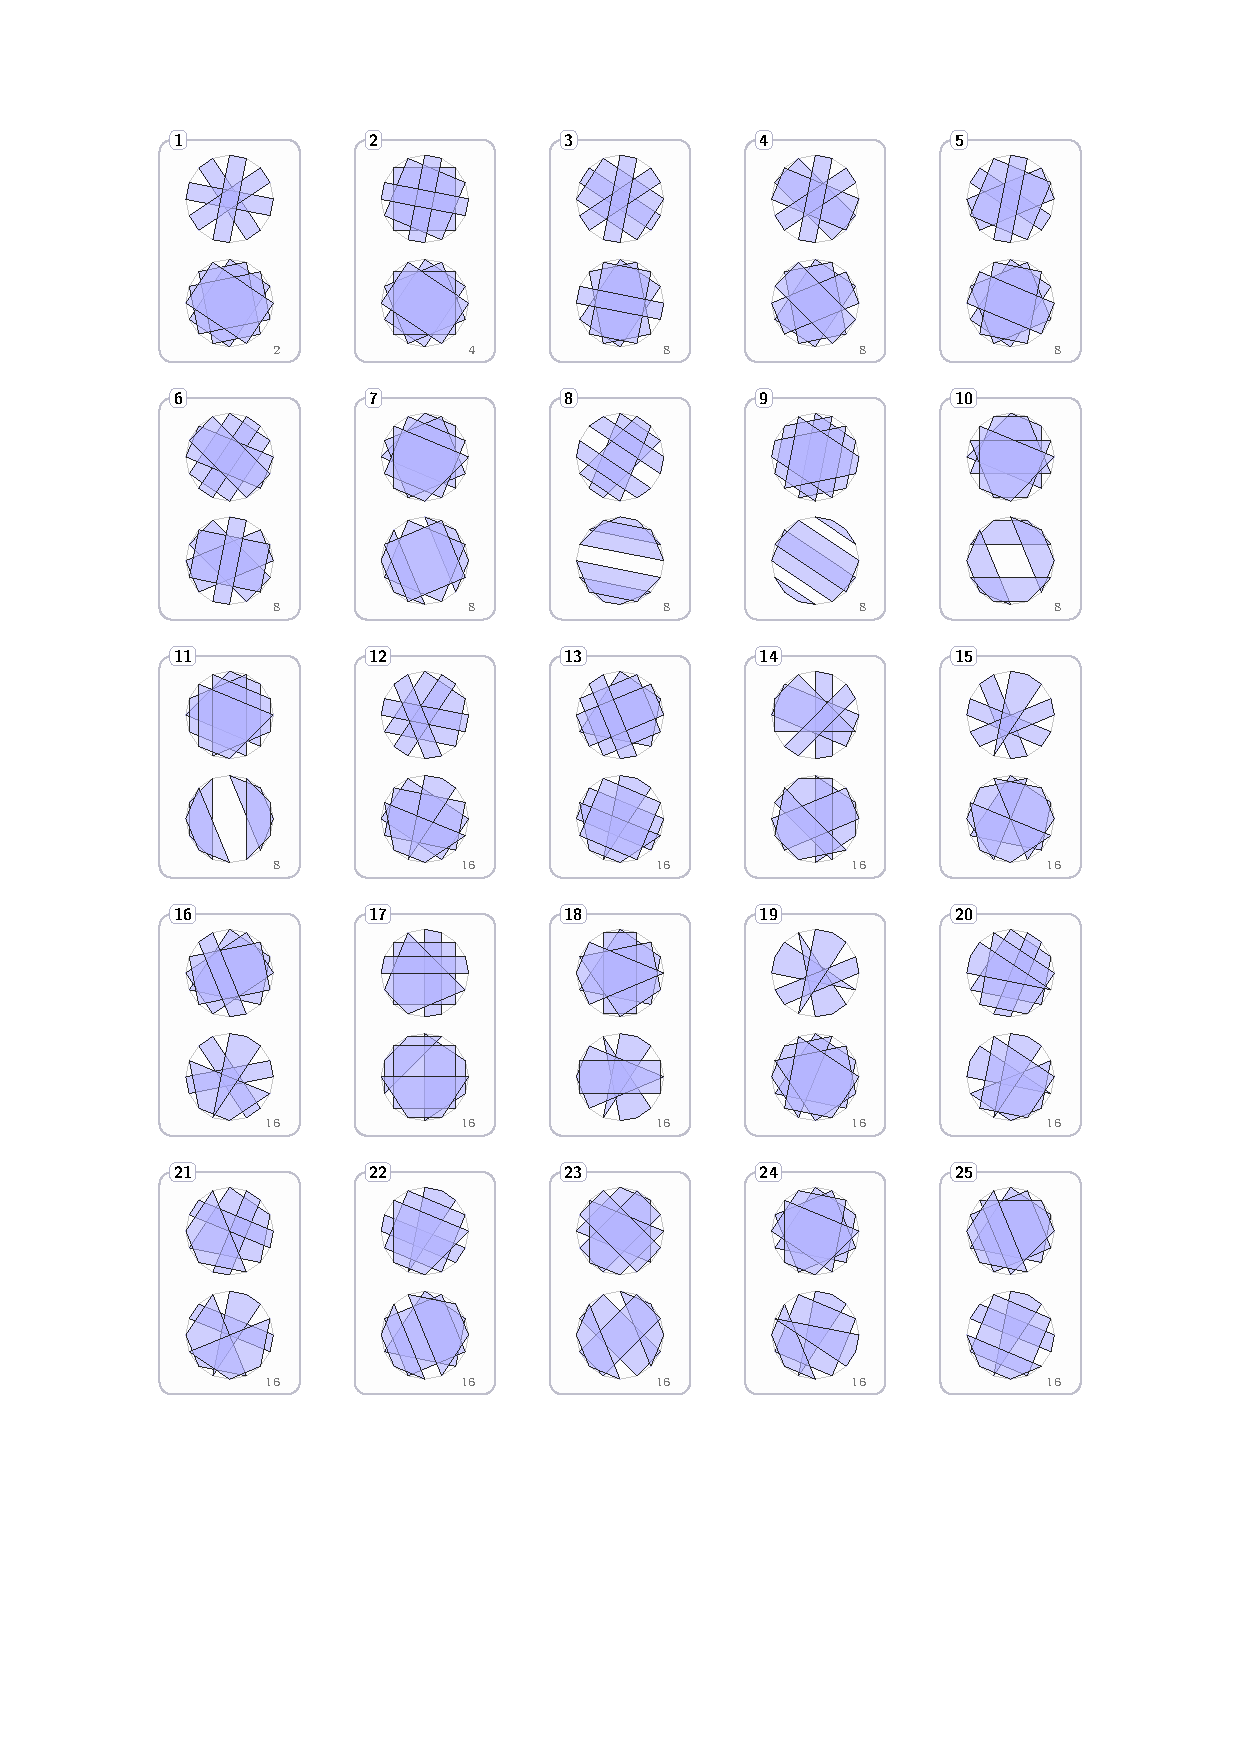
\includepdf[pages=-, pagecommand={\thispagestyle{headings}}]{plates/dimers_atlas.pdf}


\chapter{Tetramers}
\label{chap:tetramers}
% Master file for Chapter 4: The Catalogue of Tetramers
\section{Tetrameric Geometry}
\label{sec:tetramers-and-scale-models}

The vast majority of composition mosaics on $\mathbb{Z}_{16}$ (specifically, $82{,}884$ of the $83{,}488$ dihedral orbits, or $99.28\%$) gather into closed harmonic four-cycles under the Galois multiplier $\mu_3 \colon x \mapsto 3x \pmod{16}$. Theorem~\ref{thm:spectral-decomposition-z44} establishes that exactly $20{,}721$ such affine tetramers exist.

Within each tetramer cartouche, a complete orbit unfolds in a closed four-cycle:
\begin{equation}
\label{eqn:tetramer-progression}
\mu_1(O) \quad\longrightarrow\quad \mu_3(O) \quad\longrightarrow\quad \mu_7(O) \quad\longrightarrow\quad \mu_5(O) \quad\longrightarrow\quad \mu_1(O)
\end{equation}
Every step corresponds to multiplication by $3 \pmod{16}$, closing after four iterations because $3^4 \equiv 81 \equiv 1 \pmod{16}$.

\subsection{Horizontal Cartouche Geometry}

To make the algebraic sequence immediately and unambiguously readable, each tetramer unfolds in a horizontal linear cartouche ($1 \times 4$ strip). The four mosaics progress naturally from left to right across the page:
\begin{center}
\small
\begin{tabular}{cccc}
\toprule
\textbf{Position 1} & \textbf{Position 2} & \textbf{Position 3} & \textbf{Position 4} \\
\midrule
Root Orbit & First Dilation & Second Dilation (Involution) & Third Dilation (Inverse) \\
$\mu_1 \colon x \mapsto x$ & $\mu_3 \colon x \mapsto 3x$ & $\mu_7 \colon x \mapsto 7x$ & $\mu_5 \colon x \mapsto 5x$ \\
\bottomrule
\end{tabular}
\end{center}
Reading from left to right traces the exact dilation sequence:
\[
\mu_1(O) \;\xrightarrow{\mu_3}\; \mu_3(O) \;\xrightarrow{\mu_3}\; \mu_7(O) \;\xrightarrow{\mu_3}\; \mu_5(O) \;\xrightarrow{\mu_3}\; \mu_1(O)
\]
This linear orientation completely eliminates the ambiguity of two-dimensional grid layouts (where reading order conflicts with cyclic flow), making the location of the canonical root mosaic ($\mu_1$) and each subsequent modular dilation immediately discernible to the eye.

Following the standard clock-face geometry (with vertex $0$ at 12~o'clock and indices advancing clockwise), each inscribed quadrilateral is strictly convex, with its vertices circularly ordered ($v_1 < v_2 < v_3 < v_4$) to avoid self-intersecting chords, and coloured according to the two-colour symmetry taxonomy:
\begin{itemize}
    \item \textbf{Symmetric Blocks (shaded blue)}: Polygons invariant under reflection on $\mathbb{Z}_{16}$, including regular squares $(4,4,4,4)$, rectangles $(1,7,1,7)$, and symmetric trapezoids.
    \item \textbf{Chiral Blocks (shaded pink)}: Polygons lacking reflectional symmetry on $\mathbb{Z}_{16}$, occurring in enantiomorphic pairs.
\end{itemize}

\subsection{Natural Geometric Sorting}

To give the entire universe of $20{,}721$ tetramers a mathematically natural and visually striking progression, every cartouche is indexed according to a 5-tier hierarchical cascade:
\begin{enumerate}
    \item \textbf{Tier 1: Dihedral Orbit Size $|O|$}:
    Arranged in ascending order of dihedral orbit size:
    \[
    |O| \in \{4, 8, 16, 32\}
    \]
    The highest-symmetry orbits ($|O| = 4$ and $|O| = 8$) appear at the very head of the catalogue. Among all $20{,}721$ tetramers, exactly $2$ have orbit size $4$, $21$ have orbit size $8$, $622$ have orbit size $16$, and the remaining $20{,}076$ have orbit size $32$.
    
    \item \textbf{Tier 2: Symmetric Block Count $s$}:
    Within each orbit size, tetramers are sorted by the number of symmetric (achiral) blocks $s \in \{4, 3, 2, 1, 0\}$ in descending order ($4 \to 0$). This induces an unmistakable visual transition: pages begin in pure cobalt blue ($s = 4$), with pink chiral blocks appearing gradually until the final sections display completely chiral patterns ($s = 0$).
    
    \item \textbf{Tier 3: Chord Dispersion Energy $\mathcal{E}(P)$}:
    Sorted in descending order of circular chord dispersion energy:
    \[
    \mathcal{E}(P) = \sum_{B \in P} \sum_{x < y \in B} \min((y - x) \bmod 16, (x - y) \bmod 16)^2
    \]
    High energy corresponds to maximally regular, dispersed polygons with long chords; low energy corresponds to tightly clustered chords.
    
    \item \textbf{Tier 4: Canonical Stride Profile Multiset}:
    Grouping together tetramers whose inscribed quadrilaterals have identical unoriented cyclic stride profiles.
    
    \item \textbf{Tier 5: Canonical Lexicographic Tie-Breaker}:
    Canonical sorted block-set representation on $\mathbb{Z}_{16}$.
\end{enumerate}

The complete machine-readable index of all affine macro-orbits, formatted in this compact single-character notation with full cycle relabelings and chirality signatures, is preserved in the companion resource file \texttt{hexadecality\_index.txt}.

\section{The Complete Catalogue of 20721 Tetramers}
\label{sec:tetramers-catalogue}

Following the 5-tier natural sorting cascade, the complete atlas of all $20{,}721$ affine tetramers on $\mathbb{Z}_{16}$ unfolds across the following 216 plates (96 horizontal linear cartouches per page). Each cartouche presents the canonical orbit sequence $\mu_1 \to \mu_3 \to \mu_7 \to \mu_5$ from left to right. Top-left badges give the sequential tetramer index ($T_1 \dots T_{20721}$); bottom-right numerals state the shared dihedral orbit size $|O| \in \{4, 8, 16, 32\}$. The plate sequence opens with the maximal-symmetry cobalt blue configurations ($s = 4$), transitioning gracefully across descending symmetry tiers to the fully chiral pink compositions ($s = 0$).

\clearpage
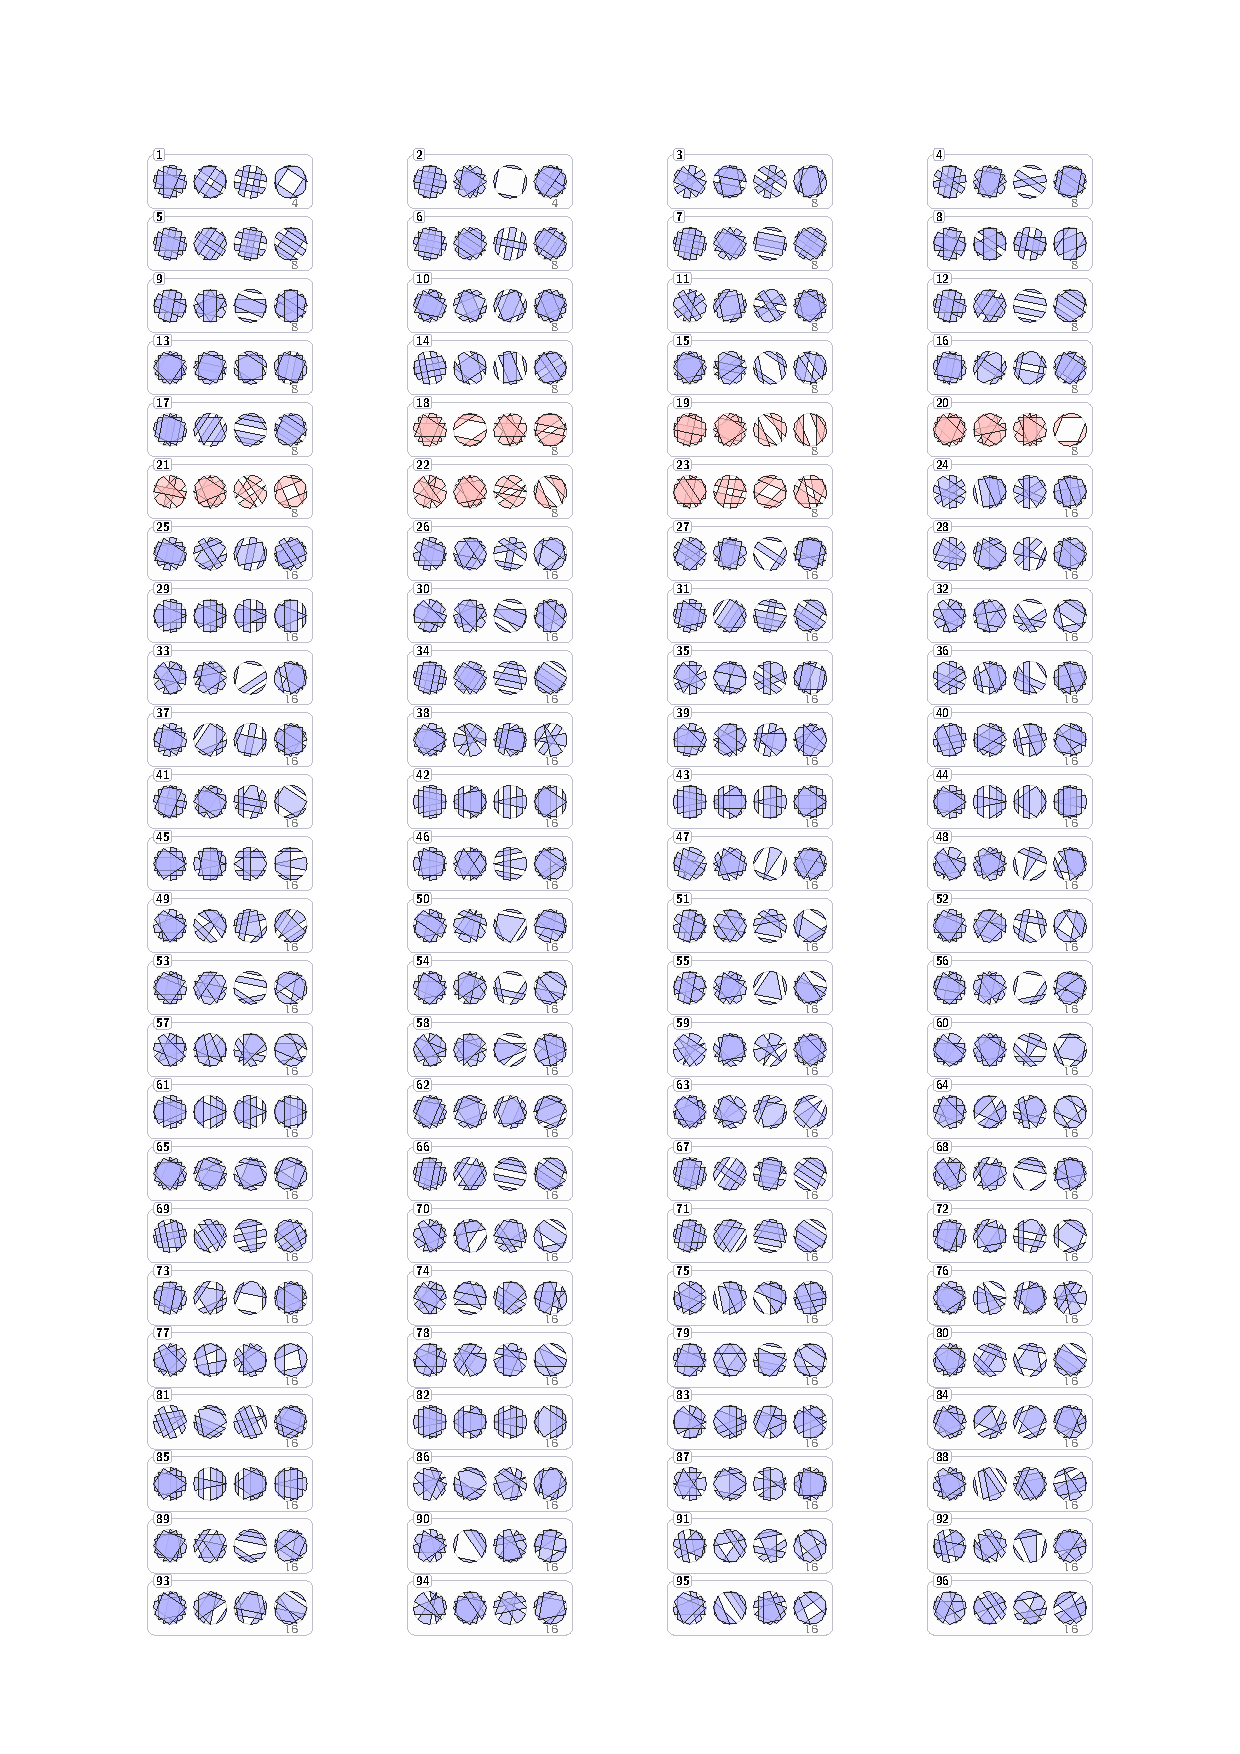
\includepdf[pages=-, pagecommand={\thispagestyle{headings}}]{plates/tetramers_atlas.pdf}


\appendix

\chapter{Smaller Universes}
\label{app:small-universes}
% Appendix: The Small Universes: D_4 and D_9
% Complete Canonical Catalogues of Sister Universes

To appreciate the vastness of the $z_4^4$ universe on $\mathbb{Z}_{16}$, it is illuminating to examine its smaller sister universes: the $D_4$ universe of 2-block partitions on $\mathbb{Z}_4$ ($z_2^2$), and the $D_9$ universe of 3-block partitions on $\mathbb{Z}_9$ ($z_3^3$). Where $\mathbb{Z}_{16}$ generates tens of thousands of orbits across multiple pages, these sibling universes are completely and exhaustively surveyable in a single glance.

\section{The \texorpdfstring{$D_4$}{D4} Universe}
\label{sec:d4-universe}

The metric arena $\mathbb{Z}_4 = \{0, 1, 2, 3\}$ represents the square. A mosaic of shape $z_2^2$ is a set partition of the four vertices into two blocks of two vertices each.

\subsection{Dihedral Orbital Enumeration}

The total number of raw equal-block partitions of shape $z_2^2$ is:
\[
\frac{1}{2!}\binom{4}{2} = \frac{6}{2} = 3
\]
These three partitions are:
\begin{align*}
P_0 &= \{\{0, 2\}, \{1, 3\}\} \\
P_1 &= \{\{0, 1\}, \{2, 3\}\} \\
P_2 &= \{\{0, 3\}, \{1, 2\}\}
\end{align*}
The dihedral group $D_4$ of order $8$ (the symmetries of the square) acts transitively on the vertices. Under this action:
\begin{itemize}
    \item $P_0$ connects opposite vertices by orthogonal interior diagonals (stride profile $(2, 2)$). It is invariant under all four rotations and all four reflections of $D_4$. Its stabiliser has full order $|\operatorname{Stab}_{D_4}(P_0)| = 8$, yielding a singleton dihedral orbit of size $|O| = 1$.
    \item $P_1$ and $P_2$ connect adjacent boundary edges (stride profile $(1, 3)$). The rotation $r \colon x \mapsto x + 1 \pmod 4$ interchanges them ($r(P_1) = P_2$, $r(P_2) = P_1$). They merge into a single dihedral orbit $\{P_1, P_2\}$ of size $|O| = 2$, with stabiliser order $4$.
\end{itemize}
Hence, there are exactly two dihedral orbits under $D_4$.

\subsection{Quotient Collapse}

The unit group of the ring $\mathbb{Z}_4$ consists of the odd residues:
\[
(\mathbb{Z}_4)^\times = \{1, 3\} = \{1, -1\}
\]
Because reflection across vertex $0$ acts on $\mathbb{Z}_4$ as $x \mapsto -x \equiv 3x \pmod 4$, the inversion multiplier $\mu_3$ is already an element of the rigid dihedral reflection group: $\mu_3 \in D_4$.

Consequently, the outer affine automorphism group collapses completely:
\[
G_{\text{macro}} = \operatorname{Aff}(\mathbb{Z}_4) / D_4 \cong (\mathbb{Z}_4)^\times / \{\pm 1\} \cong C_1
\]
The macro-quotient is the trivial group of order $1$. Every dihedral orbit is therefore an affine macro-orbit of length $1$ (a monomer). There are no dimers or tetramers.

\begin{figure}[htbp]
\centering
\input{tkz/fig_d4_universe.tkz}
\caption{\label{fig:d4-universe}The complete $D_4$ universe: the two affine monomers of shape $z_2^2$ on $\mathbb{Z}_4$. $M_1$ is the regular orthogonal cross ($|O|=1$); $M_2$ represents the parallel edges ($|O|=2$)}
\end{figure}

The complete $D_4$ catalogue consists of precisely two monomers, illustrated in Figure~\ref{fig:d4-universe}:
\begin{enumerate}
    \item \textbf{Monomer $M_1$} ($|O|=1$): The regular coset partition of the ideal $2\mathbb{Z}_4$.
    \item \textbf{Monomer $M_2$} ($|O|=2$): The parallel chord pair.
\end{enumerate}
Machine-readable relational manifests linking both monomers to \texttt{polyatlas} compositions are tabulated in \path{data/z4_mosaics.tsv} and \path{data/z4_mosaic_blocks.tsv} (see Section~\ref{sec:hexdec-relational-datasets}).

\section{The \texorpdfstring{$D_9$}{D9} Universe}
\label{sec:d9-universe}

The metric arena $\mathbb{Z}_9 = \{0, 1, \dots, 8\}$ represents the regular nonagon. A mosaic of shape $z_3^3$ partitions the nine vertices into three blocks of three vertices each (three triangles).

\subsection{The 25 Dihedral Orbits}

The raw combinatorial count of equal-block partitions of shape $z_3^3$ is:
\[
\frac{1}{3!}\binom{9}{3, 3, 3} = \frac{1}{6} \cdot \frac{9!}{(3!)^3} = \frac{1680}{6} = 280
\]
The dihedral group $D_9$ has order $|D_9| = 18$ (nine rotations and nine reflections). Under Burnside's Lemma, the number of non-equivalent dihedral orbits is:
\[
\frac{1}{18} \sum_{g \in D_9} |\operatorname{Fix}(g)| = 25
\]
These $25$ dihedral orbits stratify into four stabiliser size classes:
\begin{itemize}
    \item \textbf{Size 1 (1 orbit)}: The unique coset partition of the ideal $3\mathbb{Z}_9$:
    \[
    P_0 = \{\{0, 3, 6\}, \{1, 4, 7\}, \{2, 5, 8\}\}
    \]
    Each block is a regular equilateral triangle with stride profile $(3, 3, 3)$ (shaded blue). Invariant under all $18$ symmetries of $D_9$.
    \item \textbf{Size 3 (3 orbits)}: Three orbits with order-$6$ stabiliser $\langle r^3, s \rangle$.
    \item \textbf{Size 9 (12 orbits)}: Twelve orbits with order-$2$ bilateral reflectional stabilisers.
    \item \textbf{Size 18 (9 orbits)}: Nine fully asymmetric chiral orbits ($|\operatorname{Stab}| = 1$).
\end{itemize}
The partition sum accounts for all $280$ configurations:
\[
1 \cdot 1 + 3 \cdot 3 + 12 \cdot 9 + 9 \cdot 18 = 1 + 9 + 108 + 162 = 280
\]

\subsection{The Outer Automorphism Group \texorpdfstring{$C_3$}{C3}}

The unit group $(\mathbb{Z}_9)^\times$ consists of the six integers coprime to $9$:
\[
(\mathbb{Z}_9)^\times = \{1, 2, 4, 5, 7, 8\} \cong C_6
\]
Because reflection across vertex $0$ acts as $x \mapsto -x \equiv 8x \pmod 9$, the subgroup $\{\pm 1\} = \{1, 8\}$ lies entirely within $D_9$. Taking the quotient yields the outer macro-automorphism group:
\[
G_{\text{macro}} = \operatorname{Aff}(\mathbb{Z}_9) / D_9 \cong (\mathbb{Z}_9)^\times / \{\pm 1\} \cong C_6 / C_2 \cong C_3
\]
This outer group $G_{\text{macro}} \cong C_3$ is generated by the dilation multiplier:
\[
\mu_2 \colon x \mapsto 2x \pmod 9
\]
with cycle structure $\mu_2 \colon 1 \mapsto 2 \mapsto 4 \mapsto 8 \equiv -1 \equiv 1 \pmod{G_{\text{macro}}}$.

Because $|G_{\text{macro}}| = 3$ is a prime number, the only possible divisors are $1$ and $3$. Thus, every macro-orbit in the $D_9$ universe is either:
\begin{itemize}
    \item A \textbf{Monomer} (fixed point of length $1$).
    \item A \textbf{Trimer} (a 3-cycle under $\mu_2 \colon O \mapsto \mu_2(O) \mapsto \mu_4(O) \mapsto O$).
\end{itemize}
Applying Burnside's Lemma to the action of $C_3$ on the $25$ dihedral orbits reveals that $\mu_2$ fixes only the regular coset partition $P_0$. The remaining $25 - 1 = 24$ dihedral orbits partition into exactly $24 / 3 = 8$ Trimers!

\subsection{The Complete Inventory of Trimers}

To maintain complete methodological uniformity across universes, the nonagonal trimers are catalogued under the exact same 5-tier natural sorting cascade established for the hexadecagonal tetramers in Section~\ref{sec:tetramers-and-scale-models}:
\begin{enumerate}
    \item \textbf{Tier 1: Dihedral Orbit Size $|O|$}: Ascending order $|O| \in \{3, 9, 18\}$.
    \item \textbf{Tier 2: Symmetric Block Count $s$}: Descending order $s \in \{3, 1, 0\}$, producing the characteristic visual transition from pure cobalt blue ($s=3$) through mixed chirality ($s=1$) to full chiral pink ($s=0$).
    \item \textbf{Tier 3: Circular Chord Dispersion Energy $\mathcal{E}$}: Descending order of total chord dispersion energy.
    \item \textbf{Tier 4: Canonical Stride Profile Multiset}: Grouping by unoriented cyclic stride profiles.
    \item \textbf{Tier 5: Lexicographic Tie-Breaker}: Sorting by canonical block elements.
\end{enumerate}
Furthermore, the orientation of each 3-strip is anchored by evaluating the 5-tier key across all three cycle phases, placing the phase of highest symmetry and dispersion energy at the leading $\mu_1$ position.

The complete census of eight trimers is catalogued in Table~\ref{tab:d9-trimers}. Together with the sole monomer $M_1$, these nine cartouches constitute the entire $D_9$ universe. The visual atlas is presented in Figure~\ref{fig:d9-universe}, where each trimer is displayed as a horizontal 3-strip tracking the Galois dilation sequence $\mu_1 \to \mu_2 \to \mu_4$. Full relational block manifests connecting all $25$ dihedral comosaics to \texttt{polyatlas} are tabulated in \path{data/z9_mosaics.tsv} and \path{data/z9_mosaic_blocks.tsv}.

\begin{table}[htbp]
\centering
\footnotesize
\setlength{\tabcolsep}{4.5pt}
\begin{tabular}{cccccc}
\toprule
\textbf{Trimer} & \textbf{$|O|$} & \textbf{$s$} & \textbf{$\mathcal{E}$} & \textbf{Canonical Strides} & \textbf{Galois Dilation Cycle ($\mu_1 \to \mu_2 \to \mu_4$)} \\
\midrule
$T_1$ & 3  & 3 & 99 & $(1, 4, 4)^3$ & \texttt{/015/267/348/} \texttt{[sss]} $\to$ \texttt{/012/345/678/} $\to$ \texttt{/024/168/357/} \\
$T_2$ & 9  & 3 & 90 & $(1, 4, 4)^2, (2, 2, 5)$ & \texttt{/015/237/468/} \texttt{[sss]} $\to$ \texttt{/012/378/456/} $\to$ \texttt{/024/138/567/} \\
$T_3$ & 9  & 1 & 91 & $(1, 4, 4), (2, 3, 4)^2$ & \texttt{/015/247/368/} \texttt{[snn]} $\to$ \texttt{/012/367/458/} $\to$ \texttt{/024/178/356/} \\
$T_4$ & 9  & 1 & 85 & $(1, 3, 5)^2, (1, 4, 4)$ & \texttt{/014/256/378/} \texttt{[nns]} $\to$ \texttt{/028/134/567/} $\to$ \texttt{/047/135/268/} \\
$T_5$ & 9  & 1 & 85 & $(2, 3, 4)^2, (3, 3, 3)$ & \texttt{/025/147/368/} \texttt{[nsn]} $\to$ \texttt{/014/258/367/} $\to$ \texttt{/028/147/356/} \\
$T_6$ & 18 & 1 & 88 & $(1, 3, 5), (1, 4, 4), (2, 3, 4)$ & \texttt{/014/267/358/} \texttt{[nsn]} $\to$ \texttt{/028/167/345/} $\to$ \texttt{/047/168/235/} \\
$T_7$ & 18 & 1 & 79 & $(1, 3, 5), (2, 2, 5), (2, 3, 4)$ & \texttt{/014/268/357/} \texttt{[nns]} $\to$ \texttt{/028/156/347/} $\to$ \texttt{/047/123/568/} \\
$T_8$ & 18 & 0 & 84 & $(1, 3, 5), (2, 3, 4)^2$ & \texttt{/014/257/368/} \texttt{[nnn]} $\to$ \texttt{/028/145/367/} $\to$ \texttt{/047/128/356/} \\
\bottomrule
\end{tabular}
\caption{\label{tab:d9-trimers}The complete catalogue of eight trimers of shape $z_3^3$ on $\mathbb{Z}_9$ ordered under the 5-tier natural sorting cascade ($|O| \uparrow$, $s \downarrow$, $\mathcal{E} \downarrow$, strides, lexicographical order)}
\end{table}

\begin{figure}[p]
\centering
\input{tkz/fig_d9_universe.tkz}
\caption{\label{fig:d9-universe}The complete $D_9$ universe: the sole Monomer ($M_1$, top) and the eight Trimers ($T_1 \dots T_8$, bottom), shown as horizontal 3-strips under the Galois generator $\mu_2 \colon x \mapsto 2x \pmod 9$}
\end{figure}


\chapter{Digital Resources and Computational Toolchain}
\label{app:digital-companion}
% Appendix B: Digital Resources and Computational Toolchain

This monograph is accompanied by an open suite of machine-readable datasets, relational polygon manifests, and interactive command-line utilities. All digital artifacts are designed to facilitate computational verification, algorithmic querying, and combinatorial research into cyclic lattice composition mosaics.

\section{The Atlas Index}
\label{sec:atlas-index}

The complete inventory of all $21{,}030$ affine macro-orbits is compiled in the machine-readable dataset:
\begin{center}
\path{unimosatlas/data/hexadecality_index.txt}
\end{center}
This comprehensive index contains $21{,}065$ lines covering the entire combinatorial universe of $83{,}488$ dihedral orbits ($14$ Monomers, $295$ Dimers, and $20{,}721$ Tetramers):

\begin{enumerate}
    \item \textbf{Record Identifier}:
    Prefixed by orbit class and index: \texttt{M01}--\texttt{M14} for monomers, \texttt{D001}--\texttt{D295} for dimers, and \texttt{T00001}--\texttt{T20721} for tetramers.
    
    \item \textbf{Physical Metric Invariants}:
    Each record tabulates the dihedral orbit size $|O| \in \{1, 4, 16, 32\}$, the block bilateral symmetry count $s \in \{0, \dots, 4\}$, and the total chord energy $E$.
    
    \item \textbf{Partition-Slash Notation}:
    Partitions are rendered in compact hexadecimal slash notation, where vertices $10 \dots 15$ are represented by uppercase letters $\text{A} \dots \text{F}$. For example:
    \begin{verbatim}
    /0279/18AF/35CE/46BD/
    \end{verbatim}
    denotes the partition $\{\{0, 2, 7, 9\}, \{1, 8, 10, 15\}, \{3, 5, 12, 14\}, \{4, 6, 11, 13\}\}$.
    
    \item \textbf{Block Chirality Signatures}:
    Appended to each partition is a 4-letter signature in brackets, such as \texttt{[ssss]}, \texttt{[ssnn]}, or \texttt{[nnnn]}. Each character corresponds to one block:
    \begin{itemize}
        \item \texttt{s} (symmetric): the block possesses an internal bilateral reflection axis in $\mathbb{Z}_{16}$, rendering it achiral and non-orientable (shaded blue in plates).
        \item \texttt{n} (non-symmetric): the block lacks any internal reflection axis, rendering it intrinsically chiral (shaded pink in plates).
    \end{itemize}
    
    \item \textbf{Galois Dilation Cycle Transitions}:
    For dimers and tetramers, the line tracks the transition cycle under the affine generator $\mu_3 \colon x \mapsto 3x \pmod{16}$:
    \begin{verbatim}
    D00001 Dimer |O|=4 s=4 E=640 /028A/139B/46CE/57DF/ [ssss]
      -> /068E/179F/24AC/35BD/ [ssss]
    \end{verbatim}
\end{enumerate}

\section{The Mosaical Orbit Resolver}
\label{sec:lookup-tool}

The command-line tool \texttt{unimosatlas/tools/lookup\_mosaic.py} provides an automated resolution engine for any user-supplied set partition of $\mathbb{Z}_{16}$. 

Given an arbitrary partition string in partition-slash format, the tool:
\begin{enumerate}
    \item Verifies that the string forms a valid, non-overlapping partition of $\{0, \dots, 15\}$ into four blocks of size four.
    \item Computes the full $32$-element dihedral orbit under $D_{16}$ and extracts the lexicographical canonical representative.
    \item Identifies the stabiliser subgroup and determines the dihedral orbit size $|O| \in \{1, 4, 16, 32\}$.
    \item Calculates the chord energy $E$ and the block chirality signature.
    \item Resolves the parent macro-orbit (Monomer, Dimer, or Tetramer) and its primary catalogue index.
    \item Traces the full macro-orbit under Galois dilation $\mu_3 \colon x \mapsto 3x \pmod{16}$, printing both the geometrically dilated chord diagrams and the corresponding canonical dihedral indices.
\end{enumerate}

\begin{example}
Querying the tetramer \texttt{/0279/18AF/35CE/46BD/} yields:
{\small
\begin{verbatim}
$ lookup-mosaic "/0279/18AF/35CE/46BD/"
======================================================================
HEXADECALITY: COMPOSITION MOSAIC ORBIT & CARTOUCHE RESOLVER
======================================================================
Input Partition:       /0279/18AF/35CE/46BD/  [ssss]
Canonical Dihedral D16:/0279/18AF/35CE/46BD/  [ssss]
Dihedral Orbit Size:   |O| = 4 (Stabiliser order: 8)
Symmetric Blocks:      s = 4 of 4 (Achiral)
Chord Energy:          E = 720
----------------------------------------------------------------------
Affine Macro-Orbit Type: Tetramer (4-Cycle)

Orbital Comosaics Cycle (Physical Dilation vs Canonical Rep):
  Phase 1 (mu_1 = id) : /0279/18AF/35CE/46BD/ [ssss] (Canonical)
  Phase 2 (mu_3 = x3) : /056B/127C/38DE/49AF/ [ssss]
                        (Canonical: /016B/27CD/389E/45AF/)
  Phase 3 (mu_7 = x7) : /01EF/2345/6789/ABCD/ [ssss]
                        (Canonical: /0123/4567/89AB/CDEF/)
  Phase 4 (mu_5 = x5) : /03AD/147E/258B/69CF/ [ssss]
                        (Canonical: /0369/18BE/25CF/47AD/)
======================================================================
\end{verbatim}}
\end{example}

\section{The Relational Polygon Datasets and Embedding Manifests}
\label{sec:hexdec-relational-datasets}

To establish a bidirectional bridge between composition mosaics and the canonical inscribed polygon census of \texttt{polyatlas}, the entire combinatorial corpus across all three metric universes ($\mathbb{Z}_4$, $\mathbb{Z}_9$, and $\mathbb{Z}_{16}$) is provided as normalised, machine-readable tab-separated resource files housed in \path{unimosatlas/data/}.

\subsection{Relational Architecture and Syntax}

Each universe is structured as a relational pair:
\begin{enumerate}
    \item \textbf{Mosaic-Level Catalogue (\path{data/z*_mosaics.tsv})}:
    Tabulates the global dihedral and affine invariants ($|O|$, $|\operatorname{Stab}|$, $s$, $E$, chirality signature), the constituent polygon multiset profile, and the collective \emph{block manifest}.
    
    \item \textbf{Block-Level Relational Bridge (\path{data/z*_mosaic_blocks.tsv})}:
    Links each individual block in every canonical mosaic directly to its parent inscribed polygon class in \path{polyatlas/data/inngons.tsv}.
\end{enumerate}

Every block embedding is encoded by the standardised manifest descriptor:
\begin{equation}
\label{eqn:hexdec-block-manifest}
\text{[Class]}@\text{[Root]}[\text{Chirality}]:\text{[Realised Strides]}
\end{equation}
where \textbf{Class} denotes the parent polygon class $k\text{-}i$ defined in \texttt{polyatlas}; \textbf{Root} is the starting vertex $v_0 = \min(B_j)$ around the clock face; \textbf{Chirality} specifies the orientation sign ($+$ for direct rotational alignment, $-$ for retrograde reflection); and \textbf{Realised Strides} lists the forward perimeter strides from $v_0$ along the block.

\subsection{Multi-Universe Relational Directory}

The companion datasets span three cyclic universes:
\begin{itemize}
    \item \textbf{$D_4$ Universe ($z_2^2$ on $\mathbb{Z}_4$)}:
    \path{data/z4_mosaics.tsv} ($2$ orbits) and \path{data/z4_mosaic_blocks.tsv} ($4$ block records). Both digon classes ($2\text{-}1$ and $2\text{-}2$) are realised.
    
    \item \textbf{$D_9$ Universe ($z_3^3$ on $\mathbb{Z}_9$)}:
    \path{data/z9_mosaics.tsv} ($25$ dihedral comosaics across $9$ macro-orbits) and \path{data/z9_mosaic_blocks.tsv} ($75$ block records). All $7$ triangle classes ($3\text{-}1$ through $3\text{-}7$) are fully realised.
    
    \item \textbf{$D_{16}$ Universe ($z_4^4$ on $\mathbb{Z}_{16}$)}:
    \begin{itemize}
        \item \textbf{Primary Macro-Orbits}:
        \path{data/z16_macro_mosaics.tsv} ($21{,}030$ records) and\\
        \path{data/z16_macro_mosaic_blocks.tsv} ($84{,}120$ block records).
        \item \textbf{Exhaustive Dihedral Comosaics}:
        \path{data/z16_mosaics.tsv} ($83{,}488$ records) and\\
        \path{data/z16_mosaic_blocks.tsv} ($333{,}952$ block records).
    \end{itemize}
\end{itemize}

\subsection{The Injection Property and Cascade Filter}

Unlike unconstrained partitions, the mosaics treated here are equal-block partitions ($z_k^m$), representing structured injections into the general compositional universe:
\begin{itemize}
    \item \textbf{Enantiomorphic Realisation}: In \texttt{polyatlas}, chiral polygons appear strictly in their canonical direct orientation. In mosaics, chiral blocks appear in both direct ($+$) and retrograde ($-$) configurations (e.g.\ class $4\text{-}68$ exhibits $3{,}303$ direct and $2{,}563$ retrograde blocks across $\mathbb{Z}_{16}$).
    \item \textbf{Universal Surjectivity}: Across the complete $83{,}488$ comosaics of $\mathbb{Z}_{16}$, all $72$ tetragon classes from \texttt{polyatlas} are realised ($100\%$ coverage).
    \item \textbf{Sorting Cascade Dispersion}: In the $21{,}030$ primary macro-orbit representatives, exactly $70$ of the $72$ classes appear. Classes $4\text{-}1$ ($/0123/$, strides $111\text{D}$) and $4\text{-}3$ ($/0134/$, strides $121\text{C}$) are filtered out of the leading phase because the 5-tier natural sorting cascade prioritises high chord dispersion energy $E$, systematically shifting clustered blocks into dilated comosaic phases ($\mu_3$, $\mu_7$, or $\mu_5$).
\end{itemize}

\begin{table}[htbp]
\centering
\caption{\label{tab:hexdec-sample-manifests}Exemplar Composition Mosaics and their Relational Manifests}
\resizebox{\linewidth}{!}{%
\begin{tabular}{l c c c l l}
\toprule
Identifier & Type & $|O|$ & $s$ & Polygon Profile & Relational Embedding Manifest \\
\midrule
$M_1$ ($\mathbb{Z}_4$) & Monomer & 1 & 2 & $2 \times 2\text{-}2$ & \path{2-2@0+:22/2-2@1+:22} \\
$M_2$ ($\mathbb{Z}_4$) & Monomer & 2 & 2 & $2 \times 2\text{-}1$ & \path{2-1@0+:13/2-1@2+:13} \\
\midrule
$M_1$ ($\mathbb{Z}_9$) & Monomer & 1 & 3 & $3 \times 3\text{-}4$ & \path{3-4@0+:333/3-4@1+:333/3-4@2+:333} \\
$T_1$ ($\mathbb{Z}_9$) & Trimer & 3 & 3 & $3 \times 3\text{-}2$ & \path{3-2@0+:144/3-2@2+:414/3-2@3+:144} \\
$T_3$ ($\mathbb{Z}_9$) & Trimer & 9 & 1 & $3\text{-}2 + 2 \times 3\text{-}7$ & \path{3-2@0+:144/3-7@2+:234/3-7@3-:324} \\
\midrule
$M_{01}$ ($\mathbb{Z}_{16}$) & Monomer & 1 & 4 & $4 \times 4\text{-}28$ & \path{4-28@0+:4444/4-28@1+:4444/4-28@2+:4444/4-28@3+:4444} \\
$M_{02}$ ($\mathbb{Z}_{16}$) & Monomer & 4 & 4 & $2 \times 4\text{-}13 + 2 \times 4\text{-}27$ & \path{4-13@0+:1717/4-27@2+:5353/4-27@3+:3535/4-13@4+:1717} \\
$M_{05}$ ($\mathbb{Z}_{16}$) & Monomer & 16 & 4 & $4\text{-}13+4\text{-}22+4\text{-}27+4\text{-}28$ & \path{4-13@0+:1717/4-27@2+:3535/4-28@3+:4444/4-22@4+:2626} \\
$T_{00001}$ ($\mathbb{Z}_{16}$) & Tetramer & 4 & 4 & $4 \times 4\text{-}12$ & \path{4-12@0+:1636/4-12@2+:1636/4-12@3+:3616/4-12@4+:1636} \\
\bottomrule
\end{tabular}%
}
\end{table}


\backmatter
\chapter*{Suggested Reading}
\addcontentsline{toc}{chapter}{Suggested Reading}
\markboth{Suggested Reading}{Suggested Reading}

This monograph explores the combinatorial geometry and affine symmetries of uniform composition mosaics on $\mathbb{Z}_{16}$ ($z_4^4$), alongside its foundational square-dimension counterparts on $\mathbb{Z}_4$ and $\mathbb{Z}_9$. The selected works below offer foundational theory in affine automorphism groups, Galois multiplier decimations, distance geometry, and geometric music theory.

\section*{Affine Group Actions and Macro-Orbit Symmetries}

\begin{description}
    \item[\textbf{William Burnside (1911)}]\mbox{}\\
    \emph{Theory of Groups of Finite Order}, 2nd edition, Cambridge University Press, Cambridge.\\
    The classical exposition of the Cauchy--Frobenius orbit-counting lemma (Section~118), providing the foundational tool for Burnside cycle index evaluations under group equivalence.

    \item[\textbf{George P\'olya (1937)}]\mbox{}\\
    \emph{Kombinatorische Anzahlbestimmungen f\"ur Gruppen, Graphen und chemische Verbindungen}, \emph{Acta Mathematica}, 68(1):145--254.\\
    The fundamental theorem on weighted orbit enumeration and cycle index substitutions under permutation group actions.

    \item[\textbf{Harald Fripertinger (1997)}]\mbox{}\\
    \emph{Enumeration of isometry classes of mosaics}, \emph{Discrete Mathematics}, 176(1--3):87--98.\\
    The foundational algebraic paper formalising the classification of cyclic set partitions and mosaic isometry classes via cycle index plethysm.

    \item[\textbf{Harald Fripertinger (1999)}]\mbox{}\\
    \emph{Enumeration of mosaics}, \emph{Discrete Mathematics}, 199(1--3):49--60.\\
    Extends the enumeration of set partition equivalence classes to general group actions, covering affine normalisers and stabiliser decompositions.

    \item[\textbf{Adalbert Kerber (1999)}]\mbox{}\\
    \emph{Applied Finite Group Actions}, 2nd edition, Springer-Verlag, Berlin, Heidelberg.\\
    An exhaustive modern treatise on the constructive generation of orbits, double-coset algorithms, and cycle index polynomials of affine and projective groups.

    \item[\textbf{Emil Artin (1957)}]\mbox{}\\
    \emph{Geometric Algebra}, Interscience Publishers, New York.\\
    The standard algebraic reference on affine transformations, linear automorphisms, and multiplier structures over finite modular rings.
\end{description}

\section*{Metric Energy, Chord Dispersion, and Distance Geometry}

\begin{description}
    \item[\textbf{Isaac J. Schoenberg (1938)}]\mbox{}\\
    \emph{Metric spaces and positive definite functions}, \emph{Transactions of the American Mathematical Society}, 44(3):522--536.\\
    The classical foundation of isometric embeddings into Hilbert spaces and positive definite chordal distance kernels on circular metrics.

    \item[\textbf{Duncan M. Y. Sommerville (1909)}]\mbox{}\\
    \emph{On Certain Periodic Properties of Cyclic Compositions of Numbers}, \emph{Proceedings of the London Mathematical Society}, Second Series, 7:263--313.\\
    Early 20th-century treatise establishing the symmetry properties and periodic recurrence of cyclic integer compositions and chord strides.

    \item[\textbf{Hansraj Gupta (1979)}]\mbox{}\\
    \emph{Enumeration of Incongruent Cyclic $k$-gons}, \emph{Indian Journal of Pure and Applied Mathematics}, 10(8):964--999.\\
    Exact combinatorial classification of incongruent inscribed polygons in cyclic lattices under Euclidean rotation and reflection.
\end{description}

\section*{The Cyclic Lattice Cartography Trilogy}

\begin{description}
    \item[\textbf{Gemma Knee and Antigra Vitti (2026)}]\mbox{}\\
    \emph{The Polygonal Burnsidean: An Atlas of Inscribed Polygons from $\mathbb{Z}_1$ to $\mathbb{Z}_{16}$}, Newcastle upon Tyne.\\
    The companion volume establishing the comprehensive inventory of single inscribed polygon orbits ($k\text{-}i$) to which every constituent mosaic block is relationally anchored.

    \item[\textbf{Gemma Knee and Antigra Vitti (2026)}]\mbox{}\\
    \emph{An Atlas of Composition Mosaics: The Complete Dihedral Universe from $\mathbb{Z}_1$ to $\mathbb{Z}_8$}, Newcastle upon Tyne.\\
    The companion monograph exploring the unconstrained progression of all 509 dihedral composition mosaics across Bell-number partitions from $\mathbb{Z}_1$ to $\mathbb{Z}_8$.
\end{description}

\section*{Geometric Music Theory and Polyrhythmic Hockets}

\begin{description}
    \item[\textbf{Godfried T. Toussaint (2013)}]\mbox{}\\
    \emph{The Geometry of Musical Rhythm: What Makes a ``Good'' Rhythm Good?}, CRC Press, Boca Raton, FL.\\
    A comprehensive investigation into cyclic metric timelines, analysing maximal evenness, chordal dispersion, and Afro-Cuban timeline patterns as inscribed polygons in $\mathbb{Z}_{16}$.

    \item[\textbf{Dmitri Tymoczko (2011)}]\mbox{}\\
    \emph{A Geometry of Music: Harmony and Counterpoint in the Extended Common Practice}, Oxford University Press, New York.\\
    Geometrical formulation of musical scales, pitch-class sets, and voice leading as configurations and trajectories within quotient orbifolds under dihedral and symmetric group actions.

    \item[\textbf{Milton Babbitt (1961)}]\mbox{}\\
    \emph{Set structure as a compositional determinant}, \emph{Journal of Music Theory}, 5(1):72--94.\\
    Foundational study on the partitioning of the modular aggregate into mutually exclusive, affine-related pitch-class and rhythmic blocks.
\end{description}


\end{document}
